\section{Traditional Text Classification}
Traditional text classification provides an important reference point for the GitHub issue classification task because it offers a simple and efficient way to transform textual reports into numerical features. In this family of methods, issue text is represented as a high-dimensional sparse vector, typically using Term Frequency--Inverse Document Frequency (TF-IDF). Word n-grams can capture short expressions such as ``feature request'' or ``fails to compile'', while character n-grams can preserve useful fragments from identifiers, stack traces, file paths, package names, and version strings.

The main classical baseline in this project combines TF-IDF with Logistic Regression. The lightweight-model experiments additionally evaluate LinearSVC, Complement Naive Bayes, a hashing-based SGD classifier, and supervised fastText. fastText provides an efficient neural text-classification approach based on word and subword information \cite{joulin2017bag}. These models provide useful alternatives when training time, inference cost, and memory requirements are important.

Sparse models are attractive because they can usually be trained and evaluated much more cheaply than large pretrained encoders. Their main limitation is that they rely strongly on lexical patterns and have less ability to represent contextual meaning. Two issues expressing a similar intent with different vocabulary may therefore appear distant in sparse feature space. In this report, traditional models are used both as practical classifiers and as reference systems for evaluating the additional value of pretrained representations.

\section{Transformer Architecture}
The Transformer architecture replaces recurrent sequence processing with attention-based operations, enabling substantial parallelism during training and providing a flexible mechanism for modeling relationships between tokens \cite{vaswani2017attention}. The complete architecture contains encoder and decoder stacks; for this project, the most relevant component is the encoder because RoBERTa is an encoder-only Transformer model.

\begin{figure}[H]
    \centering
    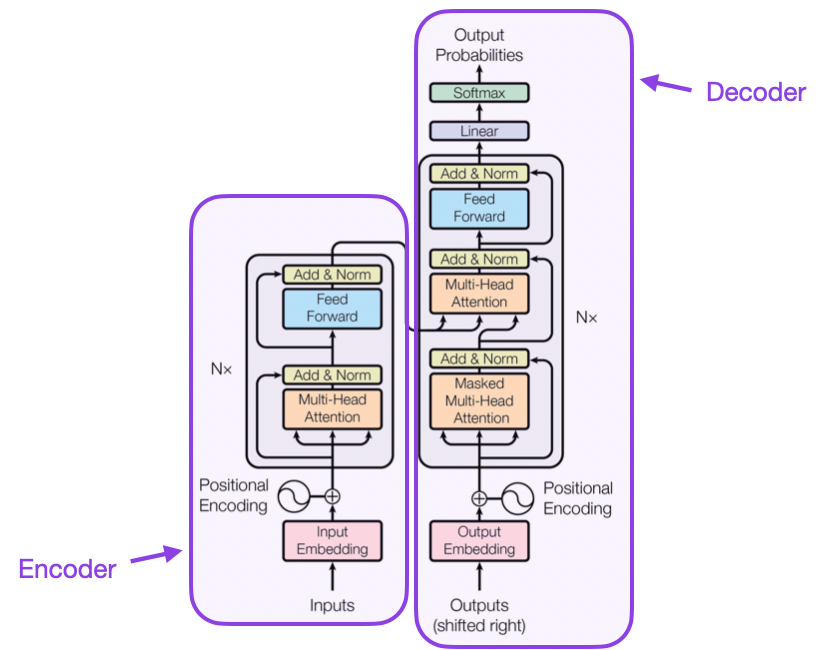
\includegraphics[width=0.52\textwidth]{image/transformer_clean.png}
    \caption{Transformer encoder--decoder architecture, adapted from Vaswani et al. \cite{vaswani2017attention}.}
    \label{fig:transformer-architecture}
\end{figure}

The main mechanisms relevant to this project are summarized below.
\begin{itemize}[leftmargin=1.5em]
    \item \textbf{Self-attention:} each token can attend to other tokens in the same sequence through query, key, and value projections. This allows the representation of a token to depend on its surrounding context.
    \item \textbf{Multi-head attention:} several attention operations are performed in parallel, allowing different heads to capture different relationships in the input.
    \item \textbf{Positional information:} because attention alone does not encode token order, positional information is added so that the model can distinguish different positions in the sequence.
    \item \textbf{Feed-forward and residual blocks:} attention layers are followed by position-wise feed-forward networks together with residual connections and normalization.
\end{itemize}

These mechanisms allow Transformer encoders to construct context-dependent token representations and make them suitable for downstream text-classification tasks.

\section{RoBERTa}
RoBERTa is a Transformer-based language model developed by revisiting and optimizing the pretraining procedure used by BERT \cite{liu2019roberta}. It retains the bidirectional Transformer encoder structure while changing several pretraining choices. In particular, RoBERTa removes the Next Sentence Prediction objective, uses dynamic masking, and is trained with more data and larger training configurations than the original BERT setup.

For downstream text classification, a pretrained RoBERTa encoder is combined with a task-specific classification head. The input is tokenized into subword units, processed by the encoder, and converted into class scores for the target labels. During full fine-tuning, both the pretrained encoder and the classification head are updated on the task data. This approach provides a direct way to adapt contextual language representations to GitHub issue classification.

\section{Low-Rank Adaptation (LoRA)}
Low-Rank Adaptation (LoRA) is a parameter-efficient fine-tuning method that adapts a pretrained model without updating all of its original parameters \cite{hu2021lora}. Instead of replacing a pretrained weight matrix $W_0$, LoRA learns a low-rank update
\begin{equation}
    \Delta W = BA,
\end{equation}
where $A$ and $B$ are smaller trainable matrices with rank $r$ much smaller than the original matrix dimensions. The forward computation can be written conceptually as
\begin{equation}
    h = W_0x + BAx.
\end{equation}

Because the pretrained weights remain frozen, only the low-rank adapters and task-specific components need to be optimized. This can reduce the number of trainable parameters and the memory required during adaptation. In this project, LoRA is evaluated as a practical alternative to full RoBERTa fine-tuning while keeping the same task and input representation.

\section{Sentence Transformers and SetFit}
Sentence Transformers are designed to produce fixed-dimensional embeddings for complete sentences or text passages. Sentence-BERT (SBERT) uses Siamese or triplet Transformer structures to produce semantically meaningful sentence representations that can be compared efficiently with similarity measures such as cosine similarity \cite{reimers2019sentencebert}.

SetFit builds on Sentence Transformers and provides a two-stage approach to text classification \cite{tunstall2022setfit}. First, a pretrained sentence encoder is adapted using contrastive learning on pairs constructed from the labeled examples. Second, the adapted encoder produces dense sentence embeddings, and a lightweight classification head is trained on those embeddings. This separation between representation learning and classification makes SetFit particularly suitable for experiments involving limited labeled data and resource-aware training.

The project evaluates two SetFit backbones: MPNet and MiniLM. MPNet provides a larger sentence-embedding model, whereas MiniLM offers a more compact alternative. Additional experiments vary the number of labeled examples and the number of contrastive-training iterations to examine data efficiency and training-cost trade-offs.
